\chapter{Конструкторский раздел}
\label{cha:design}

В данном разделе рассматривается структура программного обеспечения.

\section{Состав программного обеспечения}

Программное обеспечение состоит из загружаемого модуля ядра.

\section{Создание usb драйвера}

Для создания usb драйвера создается экземпляр структуры usb\_driver \cite{Usb_driver}. Создание экземпляра приведено на листинге \ref{lst:usb_driver}.

\begin{lstlisting}[language=c,caption=Создание экземпляра usb драйвера,label=lst:usb_driver]
static struct usb_driver tablet_driver = {
    .name       = DRIVER_NAME,
    .probe      = tablet_probe,
    .disconnect = tablet_disconnect,
    .id_table   = tablet_table,
};
\end{lstlisting}

Для ругистрации usb драйвера используется системный вызов usb\_register \cite{Usb_register}.

\section{Структура для хранения ифнормации о графическом планшете}

Для передачи данных, связанных с графическим планшетом была создана структура tablet, приведенная на листинге \ref{lst:tablet_t}.

\begin{lstlisting}[language=c,caption=Структура планшета,label=lst:tablet_t]
struct tablet {
    unsigned char     *data;
    struct input_dev  *input_dev;
    struct usb_device *usb_dev;
    struct urb        *irq;
};
typedef struct tablet tablet_t;
\end{lstlisting}

В данной структуре созданы следующие поля:

\begin{itemize}
    \item data -- данные, передаваемые планшетом при прерывании;
    \item input\_dev -- подключенный планшет;
    \item usb\_dev -- представление usb устройства;
    \item irq -- обработчик прерываний.
\end{itemize}

\section{Структура для передачи данных о прерывании}

Для того, чтобы передавать в работу из очереди данные о прерывании была создана структура container\_urb, представленная на листинге \ref{lst:container_urb}.

\begin{lstlisting}[language=c,caption=Структура для передачи данных о прерывании,label=lst:container_urb]
struct container_urb {
    struct urb *urb;
    struct work_struct work;
};

typedef struct container_urb container_urb_t;
\end{lstlisting}

В данной структуре созданы следующие поля:

\begin{itemize}
    \item urb -- обработанное прерывание;
    \item work -- текущая работа в очереди.
\end{itemize}

\section{Обработка прерываний}

На рисунке \ref{fig:urb} предствалена схема обработки прерываний графического планшета и отправка событий нажатия на клавиши клавиатуры.

\begin{figure}[H]
    \centering
    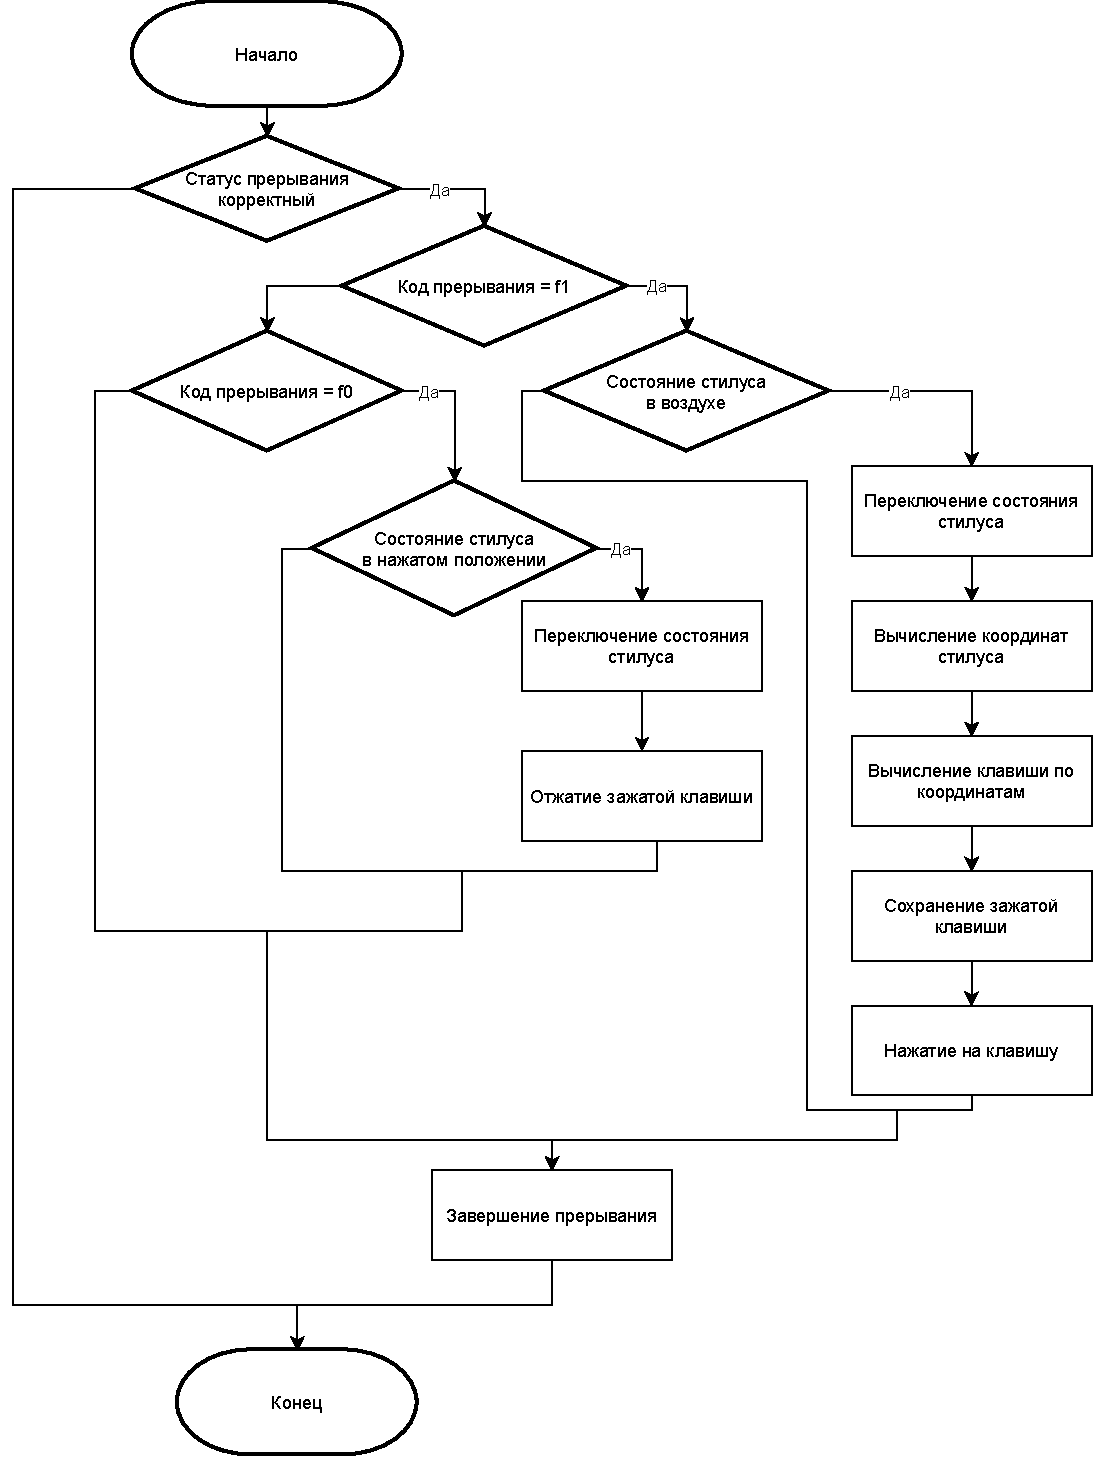
\includegraphics[width=0.9\textwidth]{img/urb.pdf}
    \caption{Обработка прерываний}
    \label{fig:urb}
\end{figure}

\section{Разделение поверхности планшета на клавиши}

Для комфортного использования модуля клавиши были расставлены на основе классической qwerty раскладки \cite{Qwerty}.

Координаты карандаша находятся в диапазоне от 0 до 1344 по оси x и от 0 до 468 по y. Поскольку координаты карандаша принимают только значения кратные 16 для оси x и кратные 9 для y, то поверхость была поделена на области размером 16 на 9. Таких областей получилось 84 на 52. Именно координаты этих областей и используются для вычисления клавиши. На рисунке \ref{fig:keyboard} представлена схема разделения поверхности планшета на клавиши клавиатуры.

\begin{figure}[H]
    \centering
    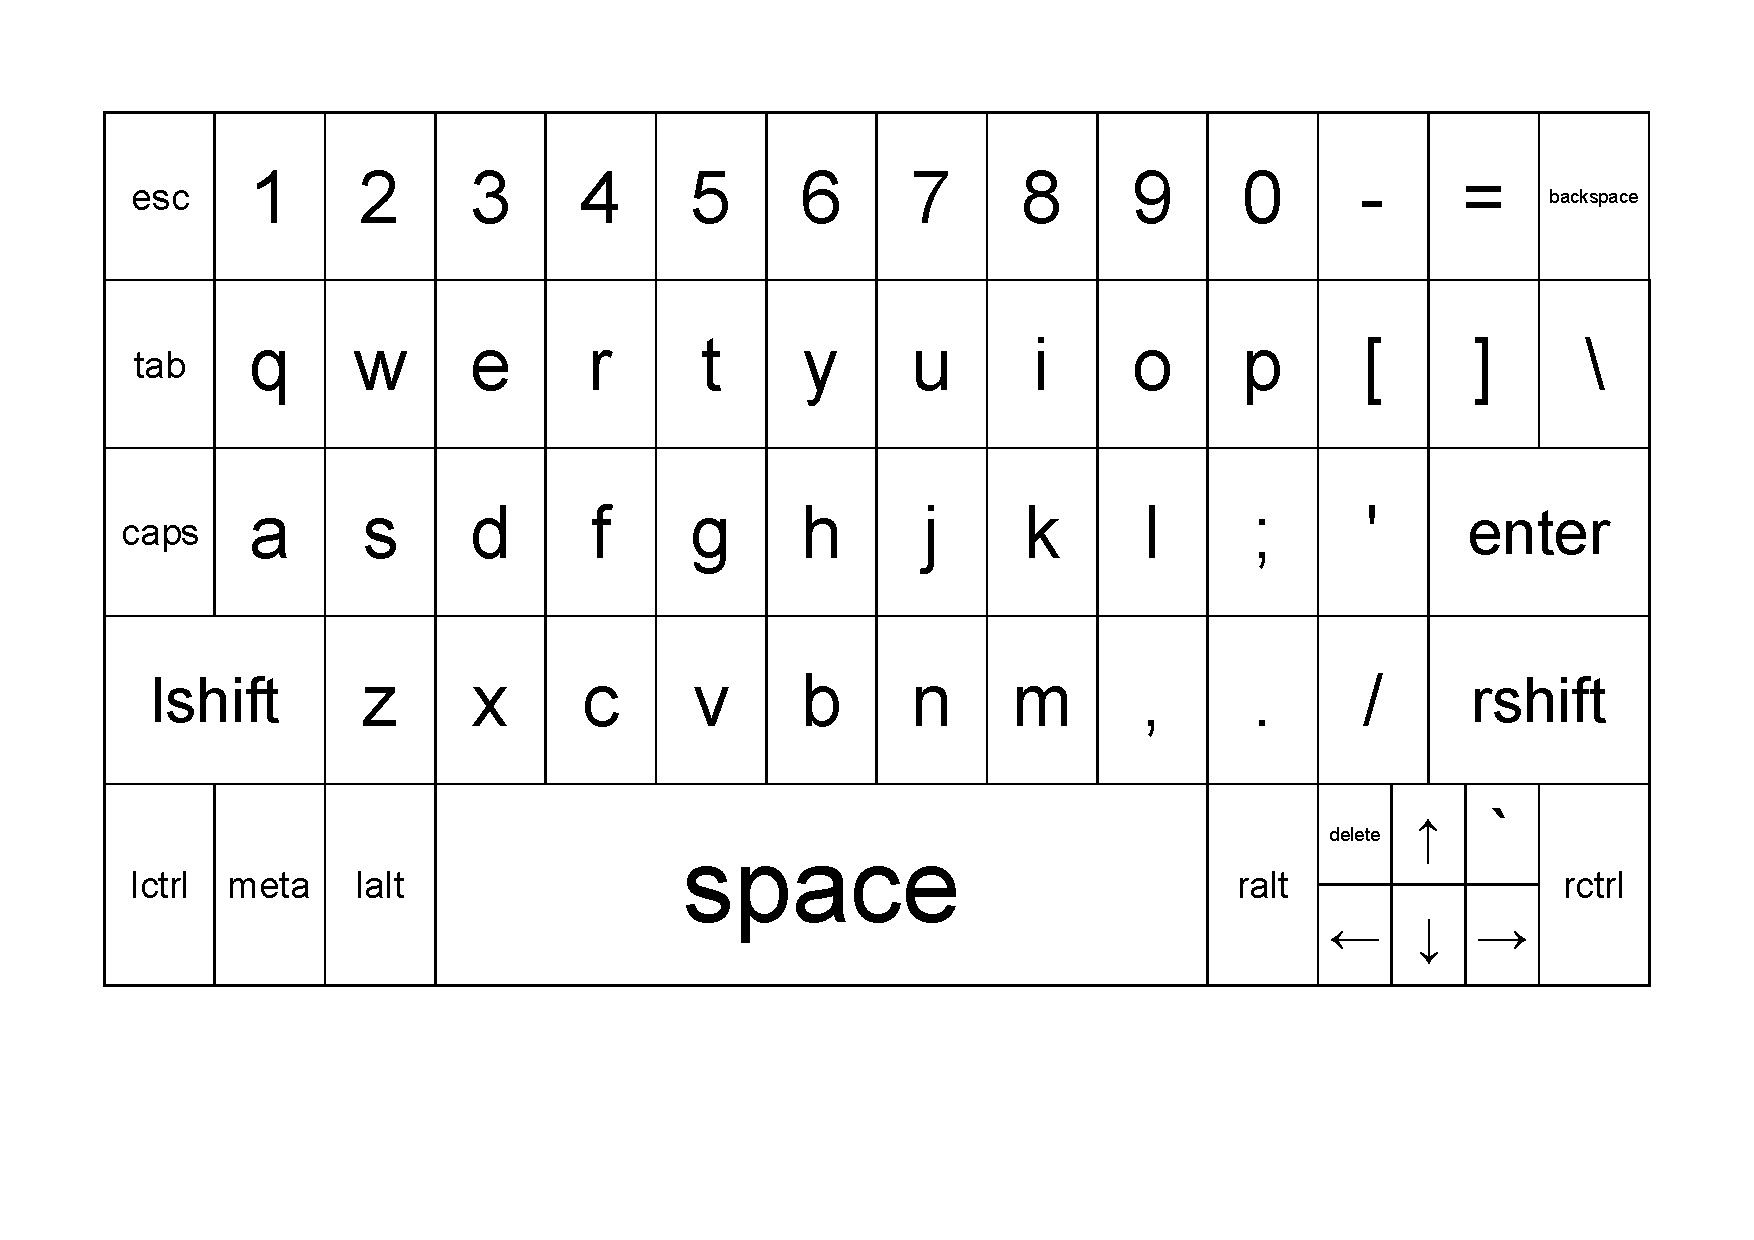
\includegraphics[trim=3cm 4cm 3cm 1.5cm, width=0.9\textwidth]{img/keyboard.pdf}
    \caption{Разделение поверхности планшета на клавиши}
    \label{fig:keyboard}
\end{figure}

\section{Вывод}

В данном разделе был рассмотрен процесс проектирования структуры программного обеспечения.
